\documentclass[12pt]{article}
\usepackage{graphicx}
\title{Programming project (no. 10)}
\author{Claus Kastorp}
\begin{document}
\maketitle
This project concerns solving the exponential function, $f(x)=exp(x)$ by means of the GSL-ODE routines (Ordinary Differential Equations). A function called exponential\_calculator is created to calculate exp(x)).\\
The crux of the situation is to create a system of differential equations which are true for the exponential as well as non-trivial, and to reduce the argument to a number $0\leq x\leq 1$ since the routines work best for small numbers.\\
First, an array y is defined as $y[0]=x,\,y[1]=\frac{df}{dx}$, and set to the function "exponential\_ode", which handles the derivatives.\\
Since $\frac{df}{dx}=f(x)$ for the exponential function, exponential\_ode returns the array of derivatives dydx[0]=dydx[1]=y[0] under the initial condition that $f(0)=f'(0)=1$.\\
The second condition, reduction of the argument, is done by recursive calling of the funciton:
\begin{itemize}
\item For x=0, f(x)=1 is returned immediately
\item For $x<0$, the function returns 1.0/exponential\_calculator(-x)
\item For $x>1$, the function defines a double Q=exponential\_calculator(x/2) and returns Q*Q
\end{itemize}
All of these calls exploit inherit properties of the exponential function.\\
The script was tested on the interval $-1\leq x\leq 3$ and are plotted in figure \ref{fig:plot} together with the exact values takes from math.h.
\\
As can be seen, the calculated values are exactly on top of the values of the function defined in math.h. Therefore, it is concluded that the function works as intended and does indeed reproduce the exponential function.\\
For large-number optimisation, a separate recursion could be called for sufficiently large numbers, such as $x>16$, which would limit the number of recursive calls.
\begin{figure}
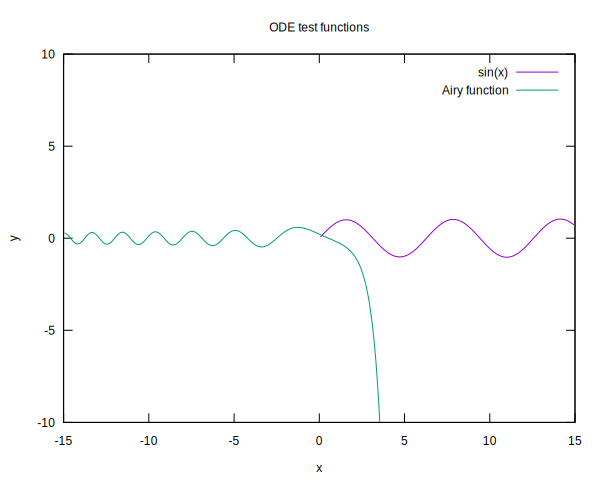
\includegraphics{plot.pdf}
\caption{Calculated vs. exact values of the exponentia function. The values returned by the script are exactly on top of the values from math.h.}
\label{fig:plot}
\end{figure}

\end{document}
